\chapter{Transformers in practice}
\label{chap:transformers_in_practice}

\begin{supportbox}{About this chapter}
We now consider a few variations of the basic transformer model, including encoder-decoder architectures, causal MHA layers, and applications to the image and audio domains.
\end{supportbox}

\section{Encoder-decoder transformers}

The model we described in Chapter \ref{chap:transformers} can be used to perform regression or classification of a given sequence. However, the original transformer \cite{vaswani2017attention} was a more complex model, designed for what are called \textbf{sequence-to-sequence} (seq2seq) tasks. In a seq2seq task, both input and output are sequences, and there is no trivial correspondence between their tokens. A notable example is \textbf{machine translation}, in which the output is the translation of the input sequence in a different language.

One possibility to build a differentiable model for seq2seq tasks is an \textbf{encoder-decoder} (ED) design \cite{sutskever2014sequence}. An ED model is composed of two blocks: an encoder that processes the input sequence to a transformed representation (possibly of a fixed dimensionality), and a decoder that autoregressively generates the output sequence conditioned on the output of the encoder. The transformer model we described before can be used to build the encoder: transformers of this type for classification are called \textbf{encoder-only} transformers. In order to build the decoder we need two additional components: a way to make the model causal (to perform autoregression), and a way to condition its computation to a separate input (the output of the encoder).

\subsection{Causal multi-head attention} \addclock

Let us consider first the problem of making the transformer block causal. The only component in which tokens interact is the MHA block. Hence, having a causal variant of MHA is enough to make the entire model causal. Remember that, for convolutions, we designed a causal variant by appropriately masking the weights in the convolutional filter. For MHA, we can mask instead all interactions between tokens that do not satisfy the causality property:
%
$$
\text{Masked-SA}(\mathbf{X})=\text{softmax}\left(\frac{\mathbf{Q}\mathbf{K}^\top {\color{drawred_l}\odot \,\mathbf{M}}}{\sqrt{k}}\right)\mathbf{V}
$$
%
It is essential to perform the masking inside the softmax. Consider the following (wrong) variant:
%
$$
\text{\color{red}\textbf{Wrong}:} \;\;\left(\text{softmax}\left(\frac{\mathbf{Q}\mathbf{K}^\top }{\sqrt{k}}\right){\color{drawred_l}\odot \,\mathbf{M}}\right)\mathbf{V}
$$
%
Because of the denominator in the softmax, all tokens participate in the computation of each token, irrespective of the later masking. Also note that setting $M_{ij}=0$ for non-causal links does not work, because $\exp(0)=1$. Hence, the correct implementation of a masked variant of MHA is to select an upper triangular matrix with $-\infty$ on the upper part, since $\exp(-\infty)=0$ as desired:
%
$$
M_{ij} =\begin{cases} -\infty & \text{ if } i > j \\ 0 & \text{ otherwise } \end{cases}
$$
%
Practically, the values can be set to a very large, negative number instead (e.g., $-10^9$).

\begin{SCfigure}
    \centering
    \hspace{1em}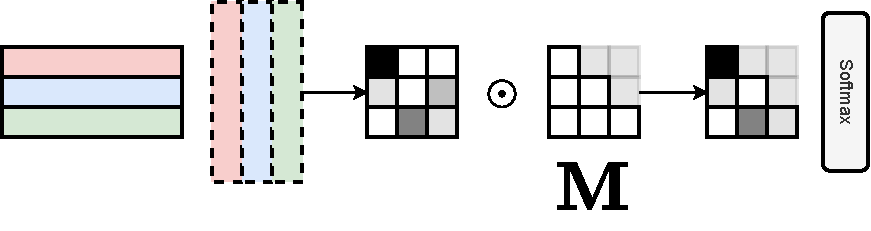
\includegraphics[width=0.7\textwidth]{images/attention_masked}
    \caption{Visual depiction of causal attention implemented with attention masking.}
    \label{fig:masked_attention}
\end{SCfigure}

\subsection{Cross-attention}

Second, let us consider the problem of making the output of the MHA layer depend on a separate block of inputs. To this end, let us rewrite the MHA operation by explicitly separating the three appearances of the input matrix:
%
$$
\text{SA}({\color{drawred}\mathbf{X}_1}, {\color{drawgreen}\mathbf{X}_2}, {\color{drawblue}\mathbf{X}_3})=\text{softmax}\left(\frac{{\color{drawred}\mathbf{X}_1}\mathbf{W}_q\mathbf{W}_k^\top{\color{drawgreen}\mathbf{X}_2^\top}}{\sqrt{k}}\right){\color{drawblue}\mathbf{X}_3}\mathbf{W}_v
$$
%
The SA layer corresponds to $\mathbf{X}_1 = \mathbf{X}_2 = \mathbf{X}_3 = \mathbf{X}$ (which, coincidentally, explains the name we gave to it). However, the formulation also works if we consider keys, values, and queries belonging to separate sets. One important case is \textbf{cross-attention} (CA), in which we assume that the keys and values are computed from a second matrix $\mathbf{Z} \sim (m,e)$:

\begin{equation}
\text{CA}(\mathbf{X}, \mathbf{Z}) = \text{SA}(\mathbf{X}, \mathbf{Z}, \mathbf{Z}) = \text{softmax}\left(\frac{\eqnmarkbox[drawred]{node}{\mathbf{X}\mathbf{W}_q\mathbf{W}_k^\top\mathbf{Z}^\top}}{\sqrt{k}}\right)\mathbf{Z}\mathbf{W}_v
\label{eq:ca}
\end{equation}
\annotate[yshift=1em]{above,right}{node}{Cross-attention between $\mathbf{X}$ and $\mathbf{Z}$}

The interpretation is that the embeddings of $\mathbf{X}$ are updated based on their similarity with a set of external (key, values) pairs provided by $\mathbf{Z}$: we say that $\mathbf{X}$ is \textit{cross-attending} on $\mathbf{Z}$. Note that this formulation is very similar to a concatenation of the two set of input tokens followed by an appropriate masking of the attention matrix.

\subsection*{Comparison with feedforward layers} \addteacup
\label{subsec:comparison_ca_mlp}

Consider a simplified variant of the cross-attention operation in \eqref{eq:ca}, in which we parameterize explicitly the keys and values matrices:\footnote{See also the discussion on the perceiver network in Section \ref{subsec:time_complexity_mha}.}
%
\begin{equation}
\text{NeuralMemory}(\mathbf{X}) = \text{softmax}\left(\frac{\mathbf{X}\mathbf{W}_q {\color{drawred}\mathbf{K}}}{\sqrt{k}}\right){\color{drawgreen}\mathbf{V}}
\label{eq:memory_layer}
\end{equation}
%
The layer is now parameterized by a query projection matrix $\mathbf{W}_q$ and by the two matrices ${\color{drawred}\mathbf{K}}$ and ${\color{drawgreen}\mathbf{V}}$. \eqref{eq:memory_layer} is called a \textbf{memory layer} \cite{sukhbaatar2015end}, in the sense that rows of the key and value matrices are used by the model to store interesting patterns to be retrieved dynamically by an attention-like operation. If we further simplify the layer by setting $\mathbf{W}_q = \mathbf{I}$, ignoring the normalization by $\sqrt{k}$, and replacing the softmax with a generic activation function $\phi$, we obtain a two-layer MLP:
%
\begin{equation}
\text{MLP}(\mathbf{X}) = \phi\left(\mathbf{X}\mathbf{K}\right)\mathbf{V}
\end{equation}
%
Hence, MLPs in transformer networks can be seen as approximating an attention operation over trainable keys and values. Visualizing the closest tokens in the training data shows human-understandable patterns \cite{geva2020transformer}.

\subsection{The complete encoder-decoder transformer}

\begin{figure}[t]
    \centering
    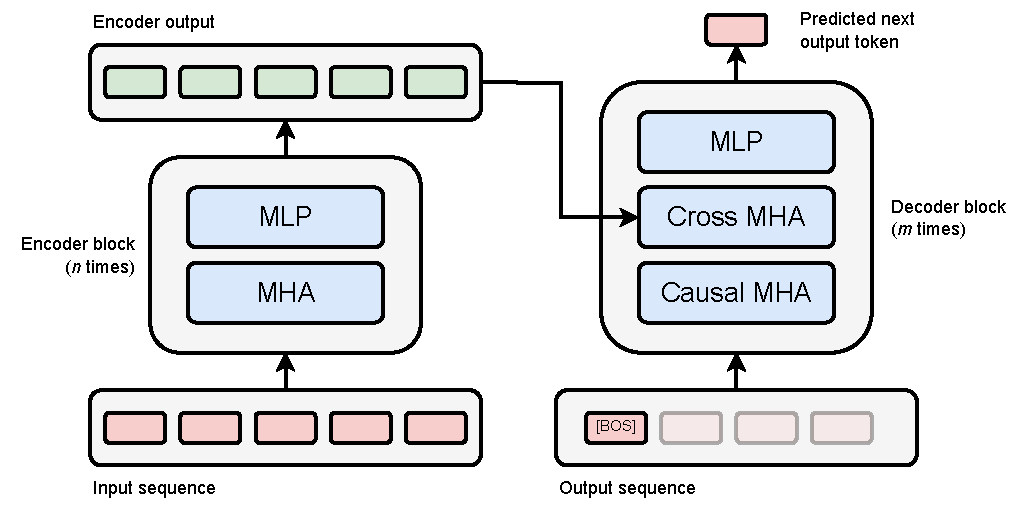
\includegraphics[width=0.8\textwidth]{images/transformer_architecture}
    \caption{Encoder-decoder architecture, adapted from \cite{vaswani2017attention}. Padded tokens in the decoder are greyed out.}
    \label{fig:transformer_model}
\end{figure}

With these two components in hand, we are ready to discuss the original transformer model, shown in Figure \ref{fig:transformer_model}.\footnote{A pedantic note: technically, Transformer (upper-cased) is a proper noun in \cite{vaswani2017attention}. In the book, I use transformer (lower-cased) to refer to any model composed primarily of attention layers.} First, the input sequence $\mathbf{X}$ is processed by a standard transformer model (called the \textbf{encoder}), providing an updated embedding sequence $\mathbf{H}$. Next, the output sequence is predicted autoregressively by another transformer model (called the \textbf{decoder}). Differently from the encoder, the decoder has three components for each block:
%
\begin{enumerate}
\item A masked variant of the MHA layer (to ensure autoregression is possible).
\item A cross-attention layer where the queries are given by the input sequence embedding $\mathbf{H}$.
\item A standard token-wise MLP.
\end{enumerate}
%
\textbf{Decoder-only} models are also possible, in which case the second block of the decoder is removed and only masked MHA and MLPs are used. Most modern LLMs are built by decoder-only models trained to autoregressively generate text tokens \cite{radford2019language}, as discussed below. In fact, encoder-decoder models have become less common with the realization that many seq2seq tasks can be solved directly with decoder-only models by concatenating the input sequence to the generated output sequence, as described in Section \ref{subsec:conditional_modelling}.

\section{Computational considerations}

\subsection{Time complexity and linear-time transformers}
\label{subsec:time_complexity_mha}

The MHA performance does not come without a cost: since every token must attend to all other tokens, its complexity is higher than a simpler convolutional operation. To understand this, we look at its complexity from two points of view: memory and time. We use a naive implementation of the SA layer for reference, shown in Box \ref{code:sa}.

\begin{mypy}{Simple implementation of the SA layer, explicitly parameterized in terms of the query, key, and value matrices.}{code:sa}
def self_attention(Q: Float[Array, "n k"], 
                   K: Float[Array, "n k"], 
                   V: Float[Array, "n v"]
                 ) -> Float[Array, "n v"]:
	return nn.softmax(Q @ K.T) @ V
\end{mypy}

Let us look first at the time complexity. The operation inside the softmax scales as $\mathcal{O}(n^2k)$ because it needs to compute $n^2$ dot products (one for each pair of tokens). Compare this to a 1D convolutional layer, which scales only linearly in the sequence length. \textit{Theoretically}, this quadratic growth in complexity can be problematic for very large sequences, which are common in, e.g., LLMs. 

This has led to the development of several strategies for speeding up autoregressive generation (e.g., speculative decoding \cite{leviathan2023fast}), as long as linear or sub-quadratic variants of transformers. As an example, we can replace the SA layer with a cross-attention layer having a \textit{trainable} set of tokens $\mathbf{Z}$, where the number of tokens can be chosen as hyper-parameter and controlled by the user. This strategy was popularized by the Perceiver architecture \cite{jaegle2021perceiver} to distill the original set of tokens into smaller latent bottlenecks. There are many alternative strategies for designing linearized transformers: we discuss a few  variants in Section \ref{subsec:mha_variants} and Chapter \ref{chap:rnns}.

Importantly, an implementation such as the one in Box \ref{code:sa} can be shown to be heavily memory-bound on modern hardware \cite{dao2022flashattention}, meaning that its compute cost is dominated by memory and I/O operations. Hence, the theoretical gains of linear-time attention variants are not correlated with actual speedup on hardware. Combined with a possible reduction in performance, this makes them less attractive than a strongly-optimized implementation of MHA, such as the one described next.

\subsection{Memory complexity and the online softmax}

In terms of memory, the implementation in Box \ref{code:sa} has also a quadratic $n^2$ complexity factor because the attention matrix $\mathbf{Q}\mathbf{K}^\top$ is fully materialized during computation. However, this is unnecessary and this complexity can be drastically reduced to a linear factor by chunking the computation in blocks and only performing the softmax normalization at the end \cite{rabe2021self}. 

To understand this, consider a single query vector $\mathbf{q}$, and suppose we split our keys and values into two blocks, which are loaded in turn in memory:

\begin{equation}
\mathbf{K} = \begin{bmatrix}\mathbf{K}_1 \\ \mathbf{K}_2 \end{bmatrix} \;,\;\;\; \mathbf{V} = \begin{bmatrix}\mathbf{V}_1 \\ \mathbf{V}_2 \end{bmatrix}
\end{equation}

If we ignore the denominator in the softmax, we can decompose the SA operation, computing the output for each chunk in turn:

\begin{equation}
\text{SA}(\mathbf{q}, \mathbf{K}, \mathbf{V}) = \frac{1}{L_1 + L_2} \left[ \mathbf{h}_1 + \mathbf{h}_2 \right]
\label{eq:attention_two_chunks}
\end{equation}

where for the two chunks $i=1,2$ we have defined two auxiliary quantities:
%
\begin{gather}
\mathbf{h}_i = \exp\left( \mathbf{K}_i\mathbf{q} \right)\mathbf{V}_i  \\
L_i = \sum_j \idx{\exp\left( \mathbf{K}_i\mathbf{q} \right)}{j}
\end{gather}
%
Remember we are loading the chunks in memory separately, hence for chunk $1$ we compute $\mathbf{h}_1$ and $L_1$; then we offload the previous chunk and we compute $\mathbf{h}_2$ and $L_2$ for chunk 2. Note that the operation is not fully-decomposable unless we keep track of the additional statistics $L_i$ (which is needed to compute the normalization coefficients of the softmax operation). More in general, for multiple chunks $i=1, \ldots, m$ we will have:

\begin{equation}
\text{SA}(\mathbf{q}, \mathbf{K}, \mathbf{V}) = \frac{1}{\sum_{i=1}^m L_i} \left[ \sum_{i=1}^m \mathbf{h}_i\right]
\label{eq:chunked_sa}
\end{equation}

Hence, we can design a simple iterative algorithm where for every block of keys and values loaded in memory, we update and store the cumulative sum of the numerator and denominator in \eqref{eq:chunked_sa}, only performing the normalization at the end. This trick (sometimes called \textit{online} softmax), combined with an IO-aware implementation and kernel fusion has led to highly memory- and compute- efficient implementations of attention such as FlashAttention-2.\footnote{\url{https://github.com/Dao-AILab/flash-attention}} Distributed implementations of attention (e.g., RingAttention \cite{liu2023ring}) can also be devised by assigning groups of queries to different devices and rotating chunks of keys and queries among the devices. Optimizing the operation for specific hardware can lead to some counter-intuitive behaviours, such as \textit{increased} speed for larger sequence lengths - see Figure \ref{fig:flash_attention}.

\begin{figure}[t]
    \centering
    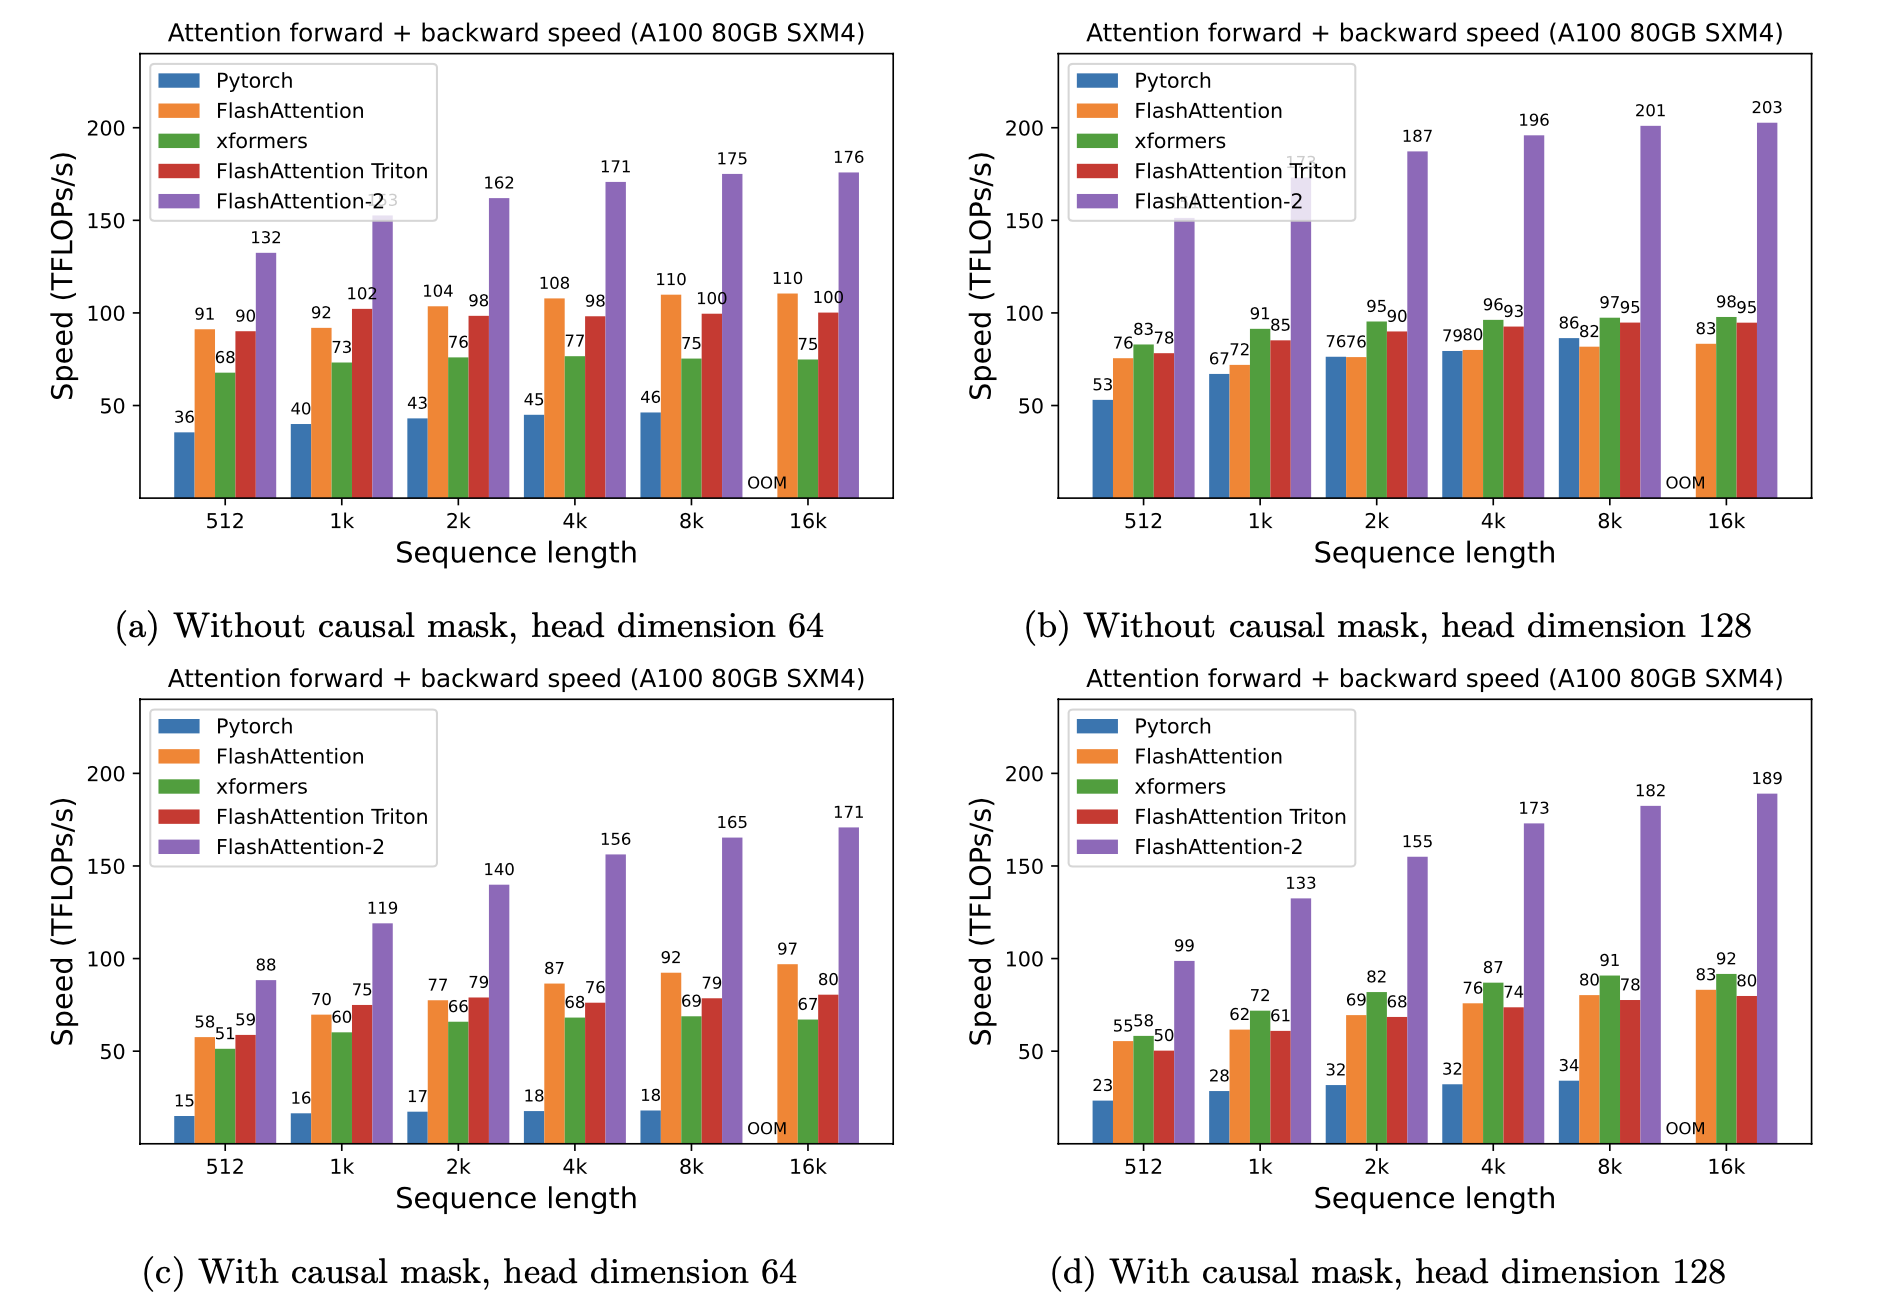
\includegraphics[width=0.7\textwidth]{images/flash2_a100_fwd_bwd_benchmark.png}
    \caption[Official benchmark of FlashAttention and FlashAttention-2 on an NVIDIA A100 GPU card.]{Official benchmark of FlashAttention and FlashAttention-2 on an NVIDIA A100 GPU card, reproduced from \url{https://github.com/Dao-AILab/flash-attention}.}
    \label{fig:flash_attention}
\end{figure}

\subsection{The KV cache}

An important implementative aspect of MHA occurs when dealing with autoregressive generation in decoder-only models. For each new token to be generated, only a new row of the attention matrix and one value token must be computed, while the rest of the attention matrix and the remaining value tokens can be stored in memory, as shown in Figure \ref{fig:kv_cache}. This is called the \textbf{KV cache} and it is a standard in most optimized implementations of MHA.

\begin{SCfigure}
    \centering
    \hspace{-0.5em}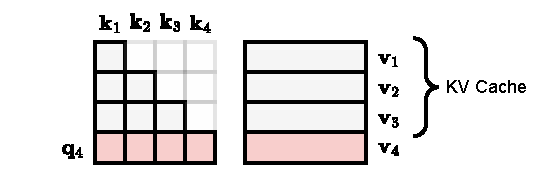
\includegraphics[width=0.6\textwidth]{images/kv_cache}
    \caption{To compute masked self-attention on a new token, most of the previous computation can be reused (in gray). This is called the \textbf{KV cache}.}
    \label{fig:kv_cache}
\end{SCfigure}

The size of the KV cache is linearly increasing in the sequence length. Once again, you can compare this to an equivalent implementation of a causal convolutional layer, where memory is upper-bounded by the size of the receptive field. Designing expressive layers with a fixed memory cost in autoregressive generation is a motivating factor for Chapter \ref{chap:rnns}.

\subsection{Transformers for images and audio} \addteacup
\label{subsec:transformers_image_audio}

Transformers were originally developed for text, and they soon became the default choice for language modeling. In particular, the popular GPT-2 model \cite{radford2019language} (and later variants) is a decoder-only architecture which is pre-trained by forecasting tokens in text sequences. Most open-source LLMs, such as LLaMa \cite{touvron2023llama}, follow a similar architecture. By constrast, BERT \cite{devlin2018bert} is another popular family of pre-trained word embeddings based on an encoder-only architecture trained to predict masked tokens (\textbf{masked language modeling}). Differently from GPT-like models, BERT-like models cannot be used to generate text but only to perform text embedding or as the first part of a fine-tuned architecture. Encoder-decoder models for language modeling also exist (e.g., the T5 family \cite{raffel2020exploring}), but they have become less popular.

From a high-level point of view, a transformer is composed of three components: a tokenization / embedding step, which converts the original input into a sequence of vectors; positional embeddings to encode information about the ordering of the original sequence; and the transformer blocks themselves. Hence, transformers for other types of data can be designed by defining the appropriate tokenization procedure and positional embeddings.

Let us consider first computer vision. Tokenizing an image at the pixel level is too expensive, because of the quadratic growth in complexity with respect to the sequence length. The core idea of Vision Transformers (ViTs, \cite{dosovitskiy2020image}) is to split the original input into non-overlapping \textbf{patches} of fixed length, which are then flattened and projected to an embedding of pre-defined size, as shown in Figure \ref{fig:image_tokenization}.

\begin{figure}[t]
    \centering
    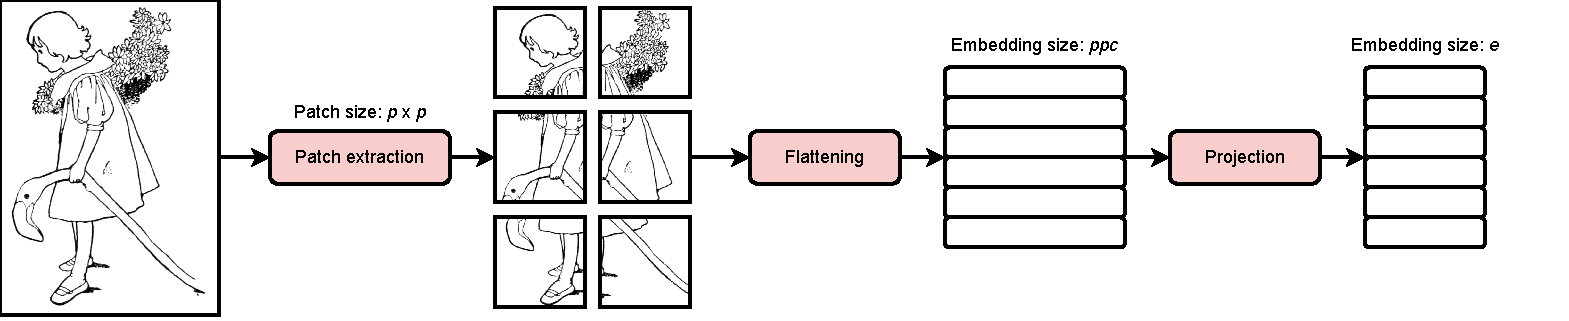
\includegraphics[width=1.0\textwidth]{images/image_tokenization}
    \caption{Image tokenization: the image is split into non-overlapping patches of shape $p \times p$ (with $p$ an hyper-parameter). Then, each patch is flattened and undergoes a further linear projection to a user-defined embedding size $e$. $c$ is the number of channels of the input image.}
    \label{fig:image_tokenization}
\end{figure}

The embedding step in Figure \ref{fig:image_tokenization} can be achieved with a convolutional layer, having stride equal to the kernel size. Alternatively, libraries like einops\footnote{\url{http://einops.rocks}} extend the einsum operation (Section \ref{sec:linear_algebra}) to allow for grouping of elements into blocks of pre-determined shape. An example is shown in Box \ref{code:einops}.

The original ViT used trainable positional embeddings along with an additional class token to perform image classification. ViTs can also be used for image generation by predicting the patches in a row-major or column-major order. In this case, we can train a separate module that converts each patch into a discrete set of tokens using, e.g., a \textbf{vector-quantized variational autoencoder} \cite{chang2022maskgit}, or we can work directly with continuous outputs \cite{tschannen2023givt}. For image generation, however, other non-autoregressive approaches such as diffusion models and flow matching tend to be preferred; we cover them in the next volume.


\begin{mypy}{einops can be used to decompose an image into patches with a simple extension of the einsum syntax.}{code:einops}
from einops import rearrange
# A batch of images
xb = torch.randn((32, 3, 64, 64)) 

# Define the operation: differently from standard einsum,
# we can split the output in blocks using brackets
op = 'b c (h ph) (w pw) -> b (h w) (ph pw c)'

# Run the operation with a given patch size
patches = rearrange(xb, op, ph=8, pw=8)
print(patches.shape) # [Out]: (32, 64, 192)
\end{mypy}

By developing proper tokenization mechanisms and positional embeddings, transformers have also been developed for audio, in particular for speech recognition. In this case, it is common to have a small 1D convolutional model (with pooling) as the tokenization block \cite{baevski2020wav2vec,radford2023robust}. For example, Wav2Vec \cite{baevski2020wav2vec} is an encoder-only model whose output is trained with an extension of the cross-entropy loss, called \textbf{connectionist temporal classification} loss \cite{graves2012connectionist}, to align the output embeddings to the transcription. Because labeled data with precise alignments is scarce, Wav2Vec models are pre-trained on large amounts of unlabeled audio with a variant of a masked language modeling loss. By contrast, Whisper \cite{radford2023robust} is an encoder-decoder model where the decoder is trained to autoregressively generate the transcription. This provides more flexibility to the model and reduces the need for strongly labeled data, but at the cost of possible \textit{hallucinations} in the transcription phase. \textbf{Neural audio codecs} can also be trained to compress audio into a sequence of discrete tokens \cite{defossez2022high}, which in turn form the basis for generative applications such as text-to-speech generation \cite{wang2023neural}.

Transformers can also be defined for time-series \cite{ansari2024chronos}, graphs (covered in the next chapter) and other types of data. The decoupling between data and architecture is also the basis for \textbf{multimodal} variants, which can take as input (or provide as output) different types of data. This is achieved by tokenizing each modality (image, audio, ...) with its appropriate tokenizer, and concatenating the different tokens together into a single sequence \cite{bordes2024introduction}. We show an example for an \textbf{image-text} model in Figure \ref{fig:multimodal_transformer}.

\begin{SCfigure}
    \centering
    \hspace{1em}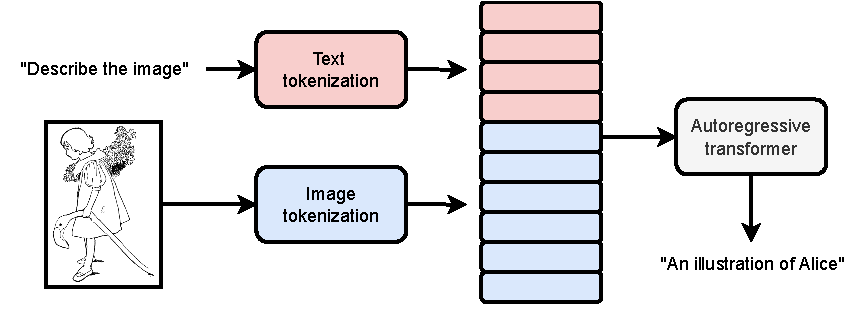
\includegraphics[width=0.65\textwidth]{images/multimodal_transformer}
    \caption{An example of a \textbf{bimodal} transformer that operates on both images and text: the outputs of the two tokenizers are concatenated and sent to the model.}
    \label{fig:multimodal_transformer}
\end{SCfigure}

\section{Variants of the transformer block}
\label{subsec:mha_variants}

We close the chapter by discussing a few interesting variation on the basic transformer block. First, several variants have been devised for very large transformers to slightly reduce the computational time or parameter’s count. As an example, \textbf{parallel blocks} \cite{dehghani2023scaling} perform the MLP and MHA operation in parallel:
%
$$
\mathbf{H} = \mathbf{H}+\text{MLP}(\mathbf{H})+\text{MHA}(\mathbf{H})
$$
%
In this way, the initial and final linear projections in the MLP and MHA layers can be fused for a more efficient implementation. As another example, \textbf{multi-query MHA} \cite{shazeer2019fast} shares the same key and value projection matrix for each head, varying only the queries.

More in general, we can replace the MHA layer with a simpler (linear complexity in the sequence length) operation, while keeping the overall structure of the transformer block, i.e., alternating token and channel mixing with layer normalization and residual connections. As an example, suppose the sequence length is fixed (e.g., for computer vision, the number of patches can be fixed a priori). In this case, the MHA layer can be replaced by an MLP operating on a single input channel, corresponding to one dimension of the embedding. This type of model is called a \textbf{mixer} model \cite{tolstikhin2021mlp} - see Figure \ref{fig:mlp_mixer}.
Ignoring the normalization operations, this can be written as alternating MLPs on transpositions of the input matrix:
%
\begin{gather}
\mathbf{H}=\text{MLP}(\mathbf{H})+\mathbf{H} \\ \mathbf{H}= \left[\text{MLP}(\mathbf{H}^\top)+\mathbf{H}^\top\right]^\top
\end{gather}
%
Other variants of the mixer model are also possible using, e.g., 1D convolutions, Fourier transforms, or pooling. In particular, in the S2-MLP \cite{yu2022s2}  model the token mixing operation is replaced by an even simpler MLP applied on a shifted version of its input. The general class of such models has been called \textbf{MetaFormers} by \cite{yu2022metaformer}.

\begin{SCfigure}
    \centering
    \hspace{1em}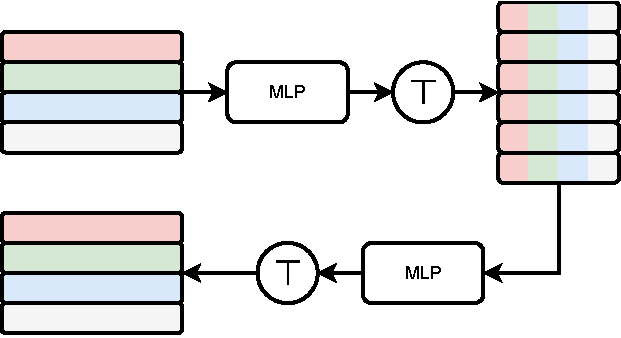
\includegraphics[width=0.55\textwidth]{images/mixer}
    \caption{Mixer block, composed of alternating MLPs on the rows and columns of the input matrix.}
    \label{fig:mlp_mixer}
\end{SCfigure}

Gated (multiplicative) interactions can also be used in the composition of the block. In this case, several blocks are executed in parallel but their output is combined via Hadamard multiplication. We can write a generic gated unit as:
%
\begin{equation}
f(\mathbf{X}) =\phi_1(\mathbf{X})\odot \phi_2(\mathbf{X})
\label{eq:glu_again}
\end{equation}
%
where $\phi_1$ and $\phi_2$ are trainable blocks. For example, with $\phi_1(\mathbf{X}) = \sigma(\mathbf{X}\mathbf{A})$ and $\phi_2(\mathbf{X})=\mathbf{X}\mathbf{B}$ we obtain the \textbf{gated linear unit} (GLU) described in Section \ref{sec:activation_functions}.

As a few representative examples, the \textbf{gMLP} model \cite{liu2021pay} uses
gated units instead of a channel mixing block in a mixer model; the \textbf{LLaMa} family of models \cite{touvron2023llama} uses GLU-like units instead of the standard MLP block; while the \textbf{gated attention unit} (GAU) \cite{hua2022transformer} uses a simpler attention-like model having a single head for $\phi_1$ and a linear projection for $\phi_2$. These designs are especially popular in some recent variants of recurrent models, discussed later on in Chapter \ref{chap:rnns}.

To simplify the design even further, the multilinear operator network (MONet) removes all activation functions to define a block which is composed only of linear projections and element-wise multiplications \cite{cheng2024multilinear}:
%
$$
\mathbf{H}=\mathbf{E}(\mathbf{A}\mathbf{X}\odot\mathbf{B}\mathbf{X}+\mathbf{D}\mathbf{X})
$$
%
where $\mathbf{E}$ is similar to the output projection in the transformer block, $\mathbf{D}\mathbf{X}$ acts as a residual connection, and $\mathbf{B}$ is implemented via a low-rank decomposition to reduce the number of parameters \cite{cheng2024multilinear}. In order to introduce token mixing, a token-shift operation is implemented in all odd-numbered blocks in the model.

\newpage
\section*{From theory to practice}

\begin{wrapfigure}{r}{3.0cm}
\vspace{-6em}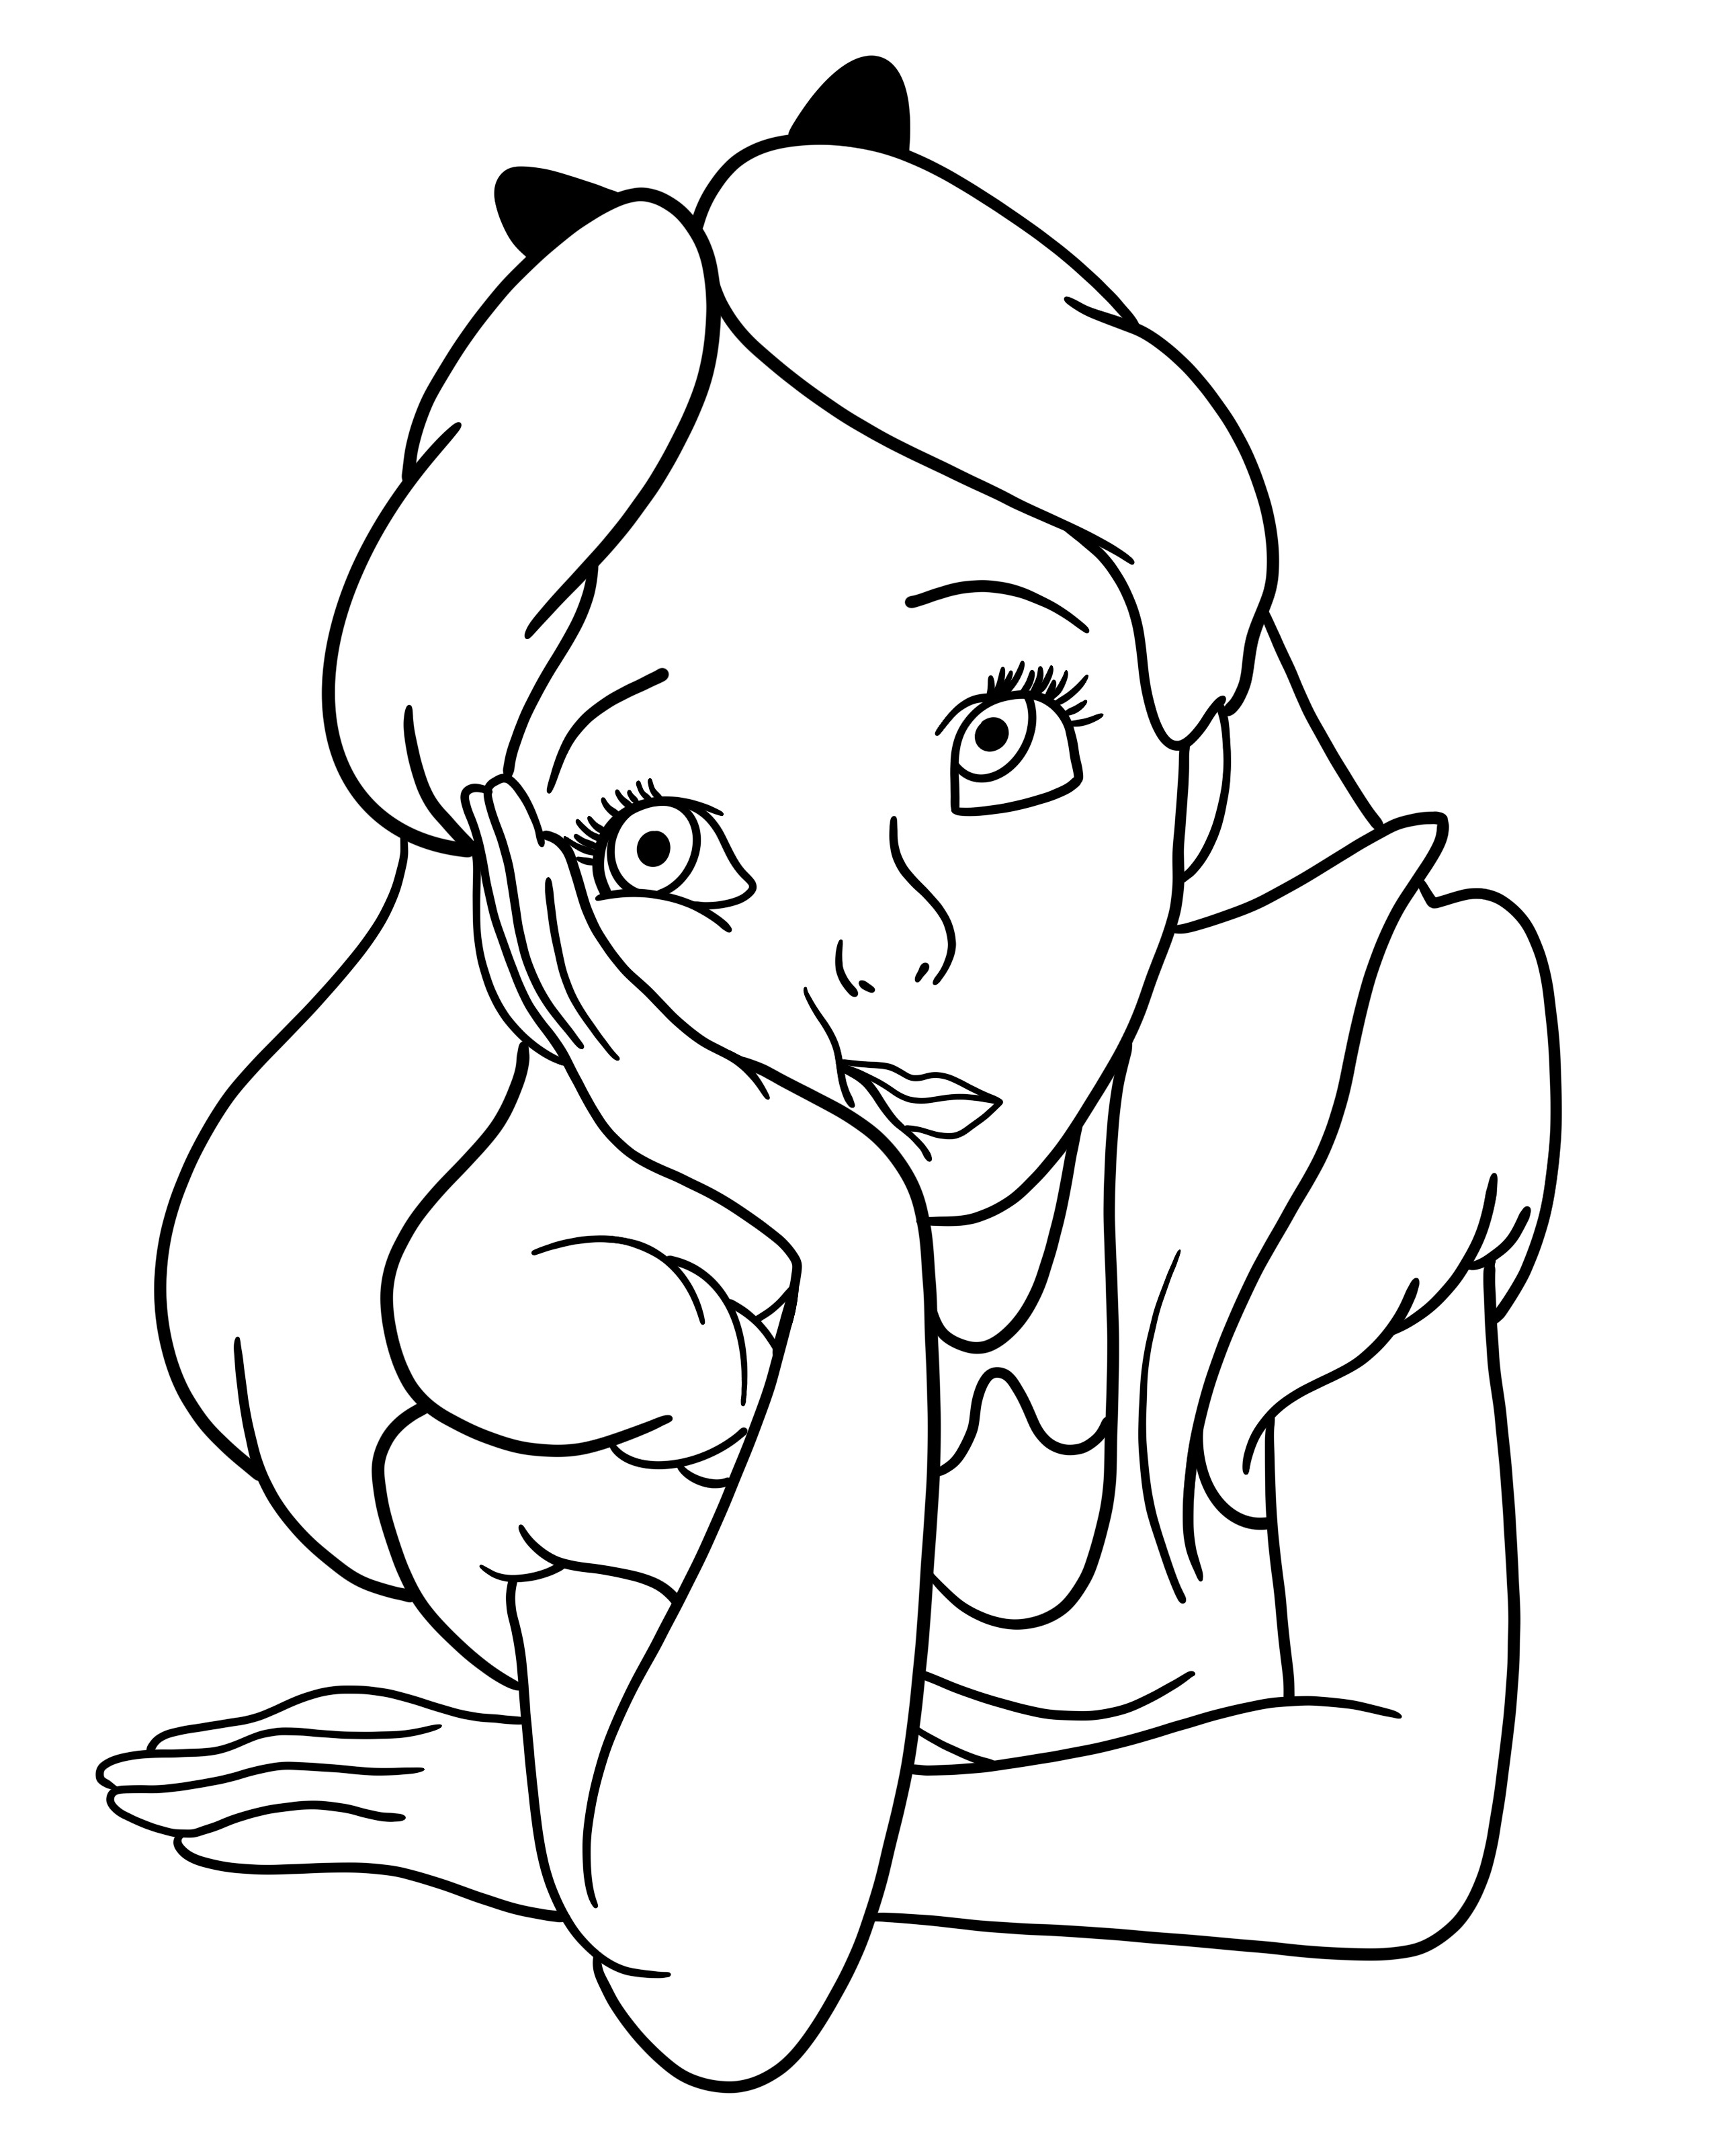
\includegraphics[width=3.0cm]{images/shutterstock_2075221579.jpg}
\vspace{-2em}
\end{wrapfigure}

There are many interesting exercises that can be done at this point -- you are almost a master in designing differentiable models! To begin, using any image classification dataset, you can try implementing from scratch a Vision Transformer as described in Section \ref{subsec:transformers_image_audio}, following \cite{dosovitskiy2020image} for choosing the hyper-parameters. Training a ViT from scratch on a small dataset is quite challenging \cite{lee2021vision,steiner2021train}, so be ready for some disappointment unless you have sufficient computational power to consider million-size datasets. You can also try a simpler variant, such as the Mixer model described in Section \ref{subsec:mha_variants}. All these exercises should be relatively simple. 

\begin{enumerate}
\item For tokenizing the image you can use Einops as in Box \ref{code:einops} or other strategies (e.g., a convolution with large stride). For small images you can also try using each pixel as token.
\item For positional embeddings, all strategies described in Section \ref{sec:positional_embeddings} are valid. The simplest one for a ViT is to initialize a matrix of \textit{trainable} embeddings, but I suggest you experiment with sinusoidal and relative embeddings as practice.
\end{enumerate}

You can also try implementing a small GPT-like model. There are many sophistications in the tokenization of text data that we do  not cover. However, the minGPT repository\footnote{\url{https://github.com/karpathy/minGPT}} is a fantastic didactic implementation that you can use as starting point.